\chapterimage{chapter_head_1.png} % Chapter heading image

\chapter{Regelbasierte Expertensysteme}



%----------------------------------------------------------------------------------------
%	Einleitung
%----------------------------------------------------------------------------------------
\section{Einleitung}
Ein Expertensystem \textit{(kurz „XPS“)} ist ein Computerprogramm, welche das Wissen spezialisierter Fachleute nachbildet. Dadurch, dass sie das Wissen über einen spezifischen Sachbereich haben, können sie Experten bei ihren täglichen Aufgaben unterstützen und sind zudem in der Lage ihr Wissen jederzeit zur Verfügung zu stellen.

\begin{center}
    \textit{
        „Expertensysteme sind Programme, mit denen das Spezialwissen und die Schlußfolgerungsfähigkeit qualifizierter Fachleute auf eng begrenzten Aufgabengebieten nachgebildet werden soll.“
    }\cite{puppe}\\
\end{center}

\noindent Es gibt unterschiedliche Arten von Expertensysteme, jedoch werden wir hier nur über die sogenannten regelbasierten Expertensysteme \textit{(engl. „Rule-based expert systems“)} sprechen.
Regelbasierte Expertensysteme schlussfolgern aus einer gegebenen Problembeschreibung eine passende Lösung.\\
Bei der Erstellung solch eines Systems sind drei wichtige Grundaufgaben zu beachten, die es lösen muss:\\

\begin{enumerate}[label=\textbf{\arabic*}.]
    \item Bereitstellen von Wissen
    \item Umgang mit Unsicherheit
    \item Verhalten erklären
\end{enumerate}



%----------------------------------------------------------------------------------------
%	Bereitstellen von Wissen
%----------------------------------------------------------------------------------------
\section{Bereitstellen von Wissen}
Um Wissen bereitstellen zu können, müssen wir erst einmal definieren, wie Wissen dargestellt wird. Außerdem müssen wir Wissen abspeichern können, deshalb werden wir uns mit dem Aufbau eines regelbasierten Expertensystems befassen und die Funktionsweise seiner wichtigsten Komponenten erläutern.
	
%------------------------------- Wie wird Wissen dargestellt? --------------------------------
%----------------------------------------------------------------------------------------------
\subsection{Wie wird Wissen dargestellt?}
Das Programm besteht aus lauter \textbf{WENN}-\textbf{DANN}-Regeln.
\begin{center}
    \textit{„\textbf{WENN} Straße nass und \textbf{WENN} Himmel bewölkt, \textbf{DANN} hat es geregnet.“}
\end{center}

\noindent Die Regeln werden vom Experten bzw. von mehreren Experten eingegeben. Da es jedoch einigen Experten schwer fällt ihr komplexes Fachwissen in obiger Form umzuformulieren, wird oft auch ein sogenannter Knowledge Engineer hinzugezogen, der das Wissen der Experten dementsprechend formalisiert und in das System einfügt.
Dieser regelbasierter Programmierstil, oft auch logischer Programmierstil genannt, steht im Kontrast zum traditionellen instruktionsbasiertem Programmierstil.
Beim instruktionsbasiertem Programmierstil besteht das Programm aus einer Abfolge von Instruktionen und Anfragen. Der Programmierer entscheidet hier was abgelaufen wird  und in welcher Reihenfolge es abgelaufen wird.
Beim regelbasiertem Programmierstil besteht das Programm aus einer Menge von Regeln. Hier entscheidet der Experte was getan werden soll und ein Regelinterpreter legt die Reihenfolge fest.\\

\begin{figure}[htp]
    \centering
    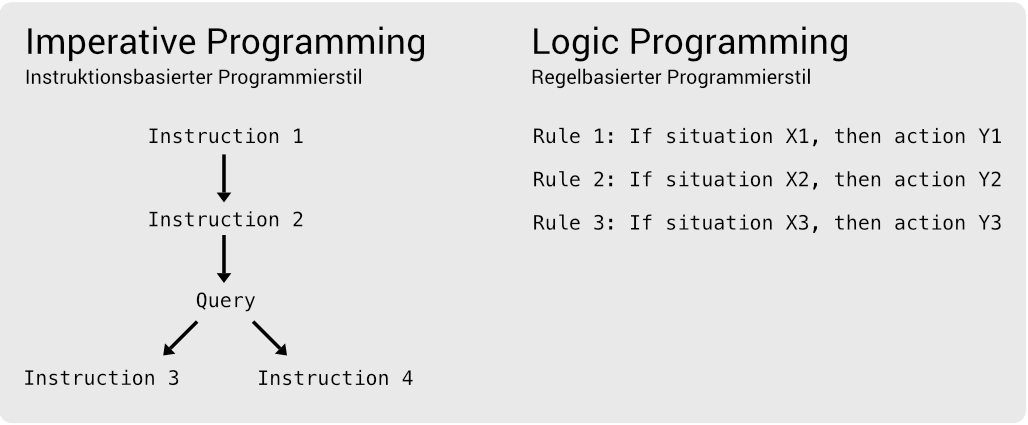
\includegraphics[width=17cm]{chapters/expertensysteme/imperative_vs_rule_based}
    \caption{Imperativer Programmierstil vs. Regelbasierter Programmierstil}
    \label{fig:programmierstil}
\end{figure}

\noindent So ein regelbasierter Ansatz hat vier wichtige Eigenschaften, die den einzelnen Komponenten des Systems zu Gute kommen. Eine Aneinanderreihung von WENN-DANN-Regeln ist\\

\begin{itemize}
    \item \textbf{Modular:} Das Wissen wird unabhängig voneinander in kleineren Regeln dargestellt.
    \item \textbf{Incrementable:} Aufgrund ihrer Modularität, können neue Regeln problemlos hinzugefügt werden.
    \item \textbf{Modifiable:} Das Ändern einer Regel beeinflusst nicht die restlichen Regeln.
    \item \textbf{Transparent:} Regeln können verwendet werden, um das Programmverhalten zu erklären.
\end{itemize}

%------------------------------- Aufbau eines Expertensystems --------------------------------
%---------------------------------------------------------------------------------------------
\subsection{Aufbau eines regelbasierten Expertensystems}
\noindent Regelbasierte Expertensysteme bestehen aus vier verschiedenen Komponenten:\\

\noindent {\fontfamily{pag}\selectfont {\small \textbf{Knowledge Base:}}}\\
Die Wissensbasis enthält das ganze Fachwissen der Experten.\\
Die ganzen WENN-DANN-Regeln sind hier gespeichert.\\

\noindent {\fontfamily{pag}\selectfont {\small \textbf{Inference Engine:}}}\\
Der Regelinterpreter bzw. der Logikkern des ganzen Systems. Mit Hilfe der Regeln aus der Knowledge Base, wird hier das Problem interpretiert, verarbeitet und gelöst.\\

\noindent {\fontfamily{pag}\selectfont {\small \textbf{Working Storage:}}}\\
Hier werden relevante Daten zur aktuellen Problemlösung zwischen gespeichert.\\

\noindent {\fontfamily{pag}\selectfont {\small \textbf{User Interface:}}}\\
Die Schnittstelle zwischen dem Benutzer und der Inference Engine.\\

\noindent Der Working Storage, die Benutzerschnittstelle sowie die Inference Engine bilden die Hülle des Systems. Die Knowledge Base soll theoretisch austauschbar sein, jedoch ist dies in der Praxis nur sehr schwer umsetzbar, denn die Inference Engine ist zu sehr auf das Wissen der Knowledge Base zugeschnitten.

\begin{figure}[H]
    \centering
    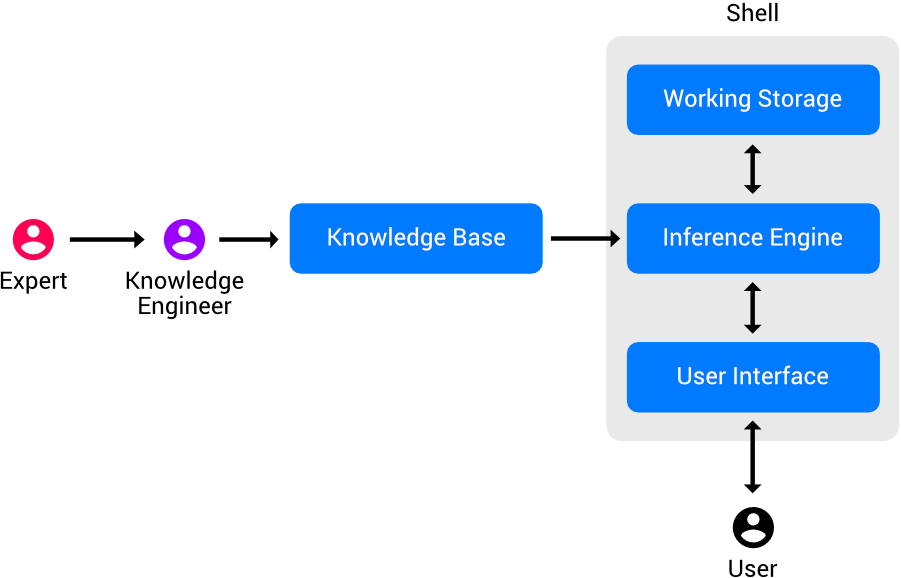
\includegraphics[width=17cm]{chapters/expertensysteme/aufbau_expertensystem}
    \caption{Aufbau eines regelbasierten Expertensystems}
    \label{fig:aufbau}
\end{figure}

%------------------------------- Wie wird Wissen abgearbeitet? --------------------------------
%----------------------------------------------------------------------------------------------
\subsection{Wie wird Wissen abgearbeitet?}
\noindent Die Inferenz der Regeln erfolgt intern über Goal Trees, auch AND-OR-Trees genannt. Ein Goal Tree weist die üblichen Baumeigenschaften auf. Das Topgoal ist die Wurzel des Baumes, dementsprechend sind die Subgoals die Teilbäume des Baumes, welche selbst wiederum Goal Trees sind. Es gibt zwei Arten von Knoten:\\

\noindent \textbf{AND-Knoten:} Hier müssen alle Teilbäume erfüllt werden.\\
\textbf{OR-Knoten:} Ein Teilbaum muss erfüllt werden.\\

\noindent Es gibt generell zwei verschiedene Ansätze um die Problemstellung zu lösen, entweder anhand des \textbf{Forward Chainings} oder seinem Gegenstück, anhand des \textbf{Backward Chainings}.



%----------------------------------------------------------------------------------------
%	Forward Chaining
%----------------------------------------------------------------------------------------
\section{Forward Chaining}
\noindent Das Forward Chaining wird auch \textbf{Data Driven Reasoning} genannt, denn man fängt mit einer gegebenen Faktenbasis \textit{(den Basiszuständen)} an. Dies sind die Blätter des Goal Trees. Von hier aus schließt man mit Hilfe der Regeln aus der Knowledge Base neue Fakten und tastet sich immer weiter vor bis man schlussendlich aus den geschlossenen Fakten eine Diagnose tätigen kann. Dies ist unser Topgoal, also die Wurzel des Goal Trees.\\

\noindent Zum Veranschaulichen ein kleines Beispiel aus der Tierwelt:\\
In der freien Natur sehen wir ein Tier, was wir identifizieren wollen. Um nun unser Problem zu lösen benutzen wir ein Expertensystem, welches mit der Methode des Forward Chaining arbeitet.
Wie oben bereits schon erwähnt fangen wir beim Forward Chaining mit einer Faktenbasis an. Auf unser Problem bezogen bedeutet dies, dass wir Beobachtungen aufstellen müssen. Zum Beispiel sehen wir, dass einige Tiere Federn haben, andere wiederum einen Schnabel. Einige leben in der Kälte, andere sind nachtaktiv. Mit Hilfe dieser Basiszustände versucht das System eine Lösung zu inferieren.\\

\begin{figure}[H]
    \centering
    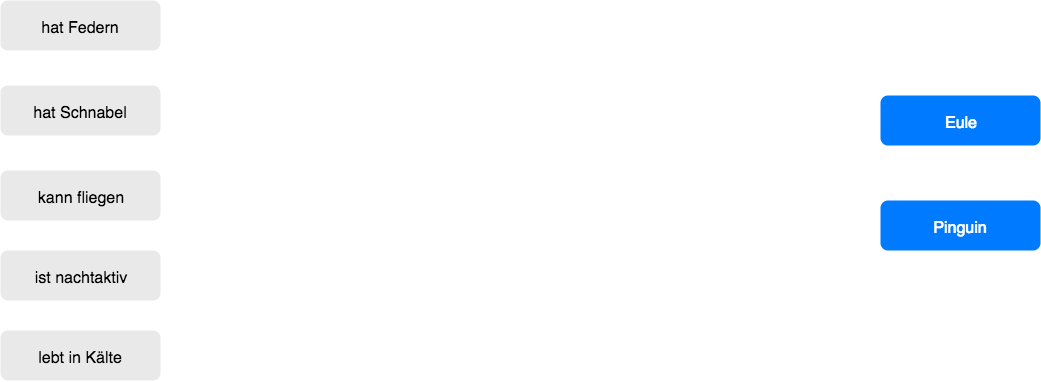
\includegraphics[width=17cm]{chapters/expertensysteme/forward_chaining/forward_chaining_1}
    \caption{Beginnen mit unserer Faktenbasis, hier links}
    \label{fig:forward_chaining_1}
\end{figure}

\noindent Mit den Regeln aus der Knowledge Base kann das System nun schrittweise zu Teillösungen voranschreiten. Die erste Regel könnte lauten: \textbf{WENN} Federn und \textbf{WENN} Schnabel, \textbf{DANN} Vogel.
\begin{figure}[H]
    \centering
    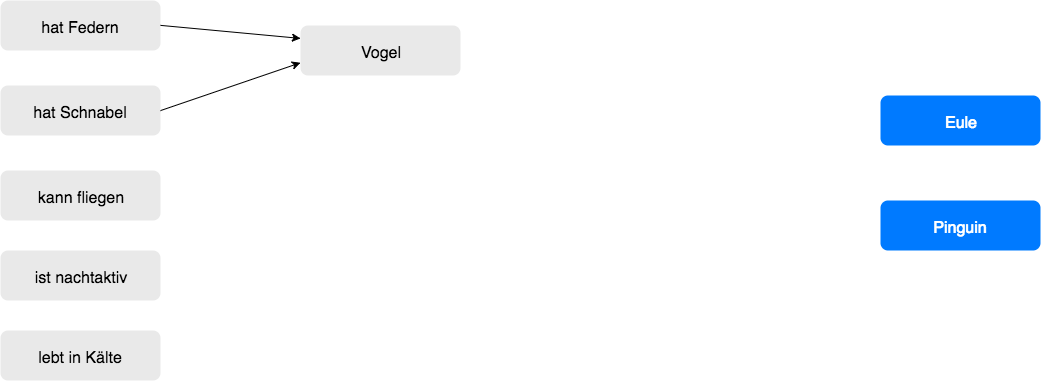
\includegraphics[width=17cm]{chapters/expertensysteme/forward_chaining/forward_chaining_2}
    \caption{Neue Teillösungen inferieren}
    \label{fig:forward_chaining_2}
\end{figure}

\noindent Eine andere Regel könnte lauten: \textbf{WENN} Vogel und \textbf{WENN} fliegen, \textbf{DANN} flugfähiger Vogel.
\begin{figure}[H]
    \centering
    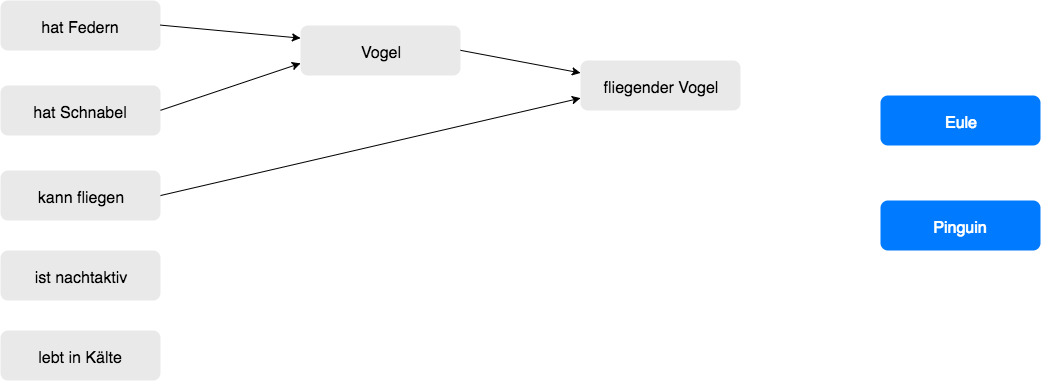
\includegraphics[width=17cm]{chapters/expertensysteme/forward_chaining/forward_chaining_3}
    \caption{Weitere Teillösung inferieren}
    \label{fig:forward_chaining_3}
\end{figure}

\clearpage
\noindent Eine weitere Regel könnte lauten: \textbf{WENN} fliegender Vogel und \textbf{WENN} nachtaktiv, \textbf{DANN} Eule. Somit hat unser Expertensystem von unseren anfänglichen Beobachtungen geschlussfolgert, dass es sich um eine Eule handeln muss.
\begin{figure}[H]
    \centering
    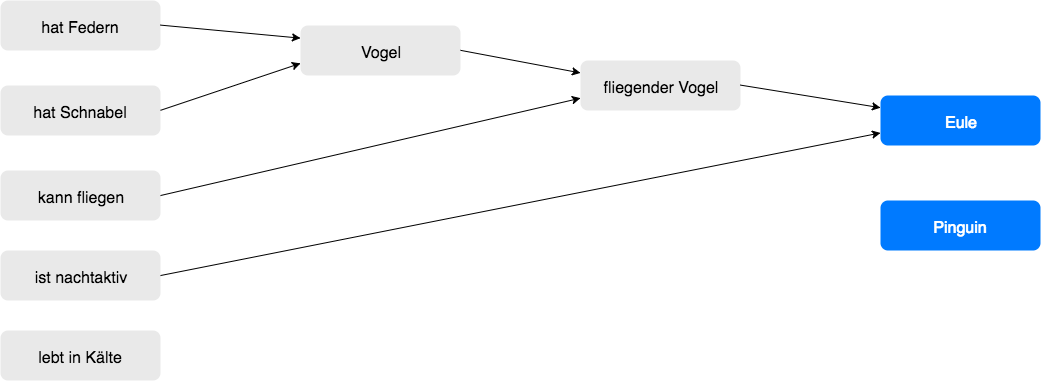
\includegraphics[width=17cm]{chapters/expertensysteme/forward_chaining/forward_chaining_4}
    \caption{Topgoal erreicht}
    \label{fig:forward_chaining_4}
\end{figure}

\noindent Würden wir nun ein weiteres Tier sehen und wieder unser Expertensystem fragen, könnte das ganze so aussehen:
\begin{figure}[H]
    \centering
    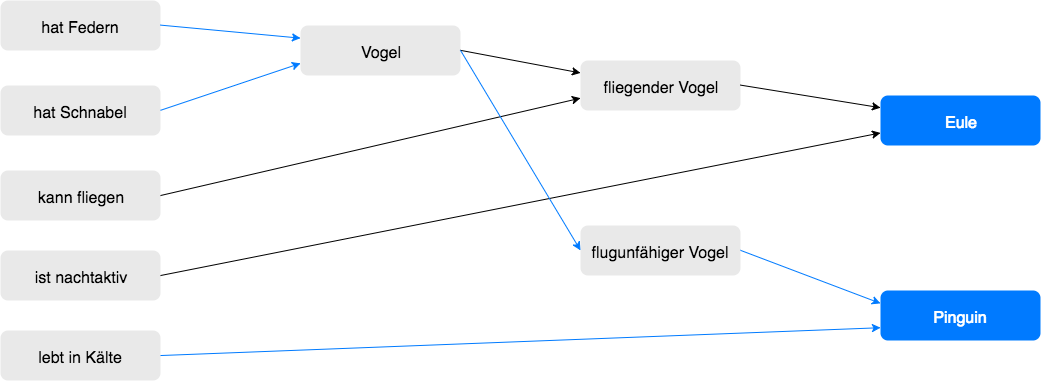
\includegraphics[width=17cm]{chapters/expertensysteme/forward_chaining/forward_chaining_5}
    \caption{Von unserer Faktenbasis inferiert das System, dass es sich um einen Pinguion handelt.}
    \label{fig:forward_chaining_5}
\end{figure}

\noindent Das Forward Chaining ist anwendbar auf Probleme mit nicht aufzählbaren Lösungen. In der Realität wird Forward Chaining daher in Design- und Konfigurationssysteme genutzt.



%----------------------------------------------------------------------------------------
%	Backward Chaining
%----------------------------------------------------------------------------------------
\section{Backward Chaining}
Backward Chaining ist wie vorher schon erwähnt das Gegenstück zum Forward Chaining. Hier beginnt man beim Topgoal und zerlegt dieses in die ursprünglichen Subgoals. Da die Subgoals prinzipiell wieder Topgoals sind zerlegt man diese auch wieder in Subgoal. Dies macht man solange bis man wieder bei den Blättern, also den Fakten angelangt ist. Man kann dazu auch sagen: Das System inferiert von den Hauptlösung zur Teillösung. Diese Teillösungen werden dabei im Working Storage gespeichert. Nun wird dies wieder an unserem bekannten Beispiel mit Eule und Pinguin illustriert.

\subsection*{Beispiel}
\begin{figure}[H]
    \centering
    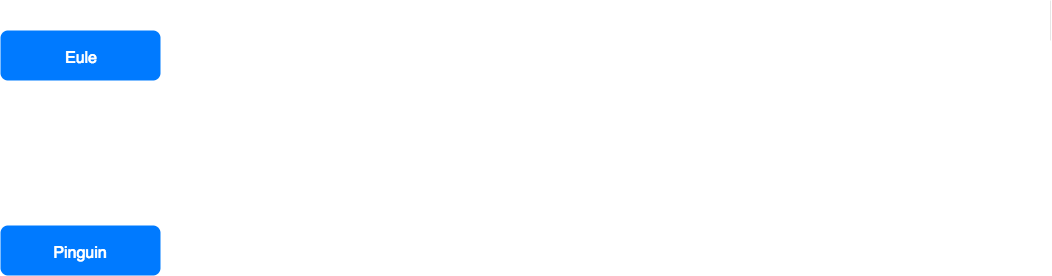
\includegraphics[width=17cm]{chapters/expertensysteme/backward_chaining/backward_chaining_1}
    \label{fig:backward_chaining_1}
\end{figure}

Wir haben nun die beiden Topgoals Eule und Pinguin gegeben. Nun möchten wir wieder zu den Teillösungen gelangen. Dies geschieht wie auch beim Forward Chaining mit den Wenn-Dann Regeln. In diesem Beispiel wäre die erste Regel:

Wenn Eule, dann kann fliegen und ist nachtaktiv

\begin{figure}[H]
    \centering
    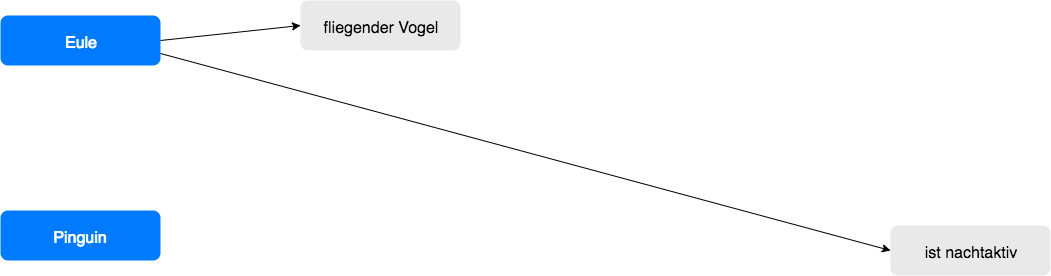
\includegraphics[width=17cm]{chapters/expertensysteme/backward_chaining/backward_chaining_2}
    \label{fig:backward_chaining_2}
\end{figure}

Dies macht man nun solange bis man wieder bei der Faktenbasis ist.

\begin{figure}[H]
    \centering
    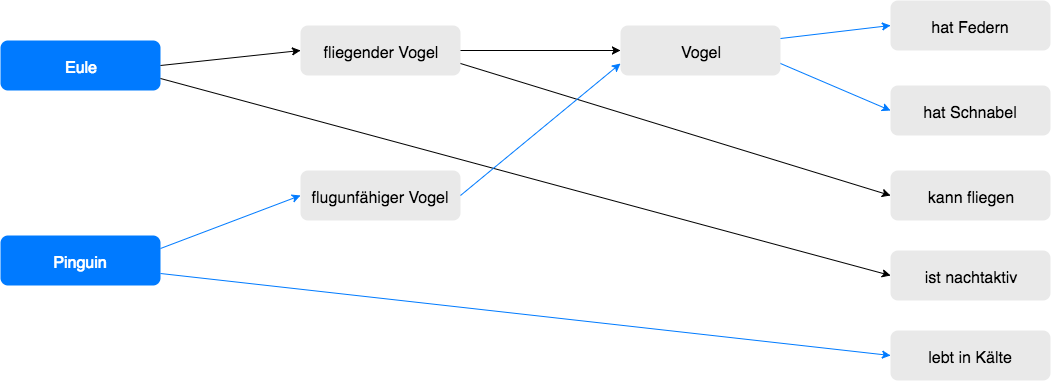
\includegraphics[width=17cm]{chapters/expertensysteme/backward_chaining/backward_chaining_3}
    \label{fig:backward_chaining_3}
\end{figure}

\noindent Diese Art von regelbasierten Expertensystem ist anwendbar auf Probleme mit strukturierter Selektion und auf Probleme, die aufzählbare Lösungen haben. Hier könnte sich die Frage stellen: Warum nur auf Probleme mit aufzählbaren Lösungen? Diese Frage beantwortet sich fast schon von allein, da jede Lösung mindestens eine Regel haben muss.

\noindent In der Realität wird Backward Chaining daher in Identifaktions- und Diagnosesysteme zum Einsatz.


%----------------------------------------------------------------------------------------
%	Umgang mit Unsicherheit
%----------------------------------------------------------------------------------------
\section{Umgang mit Unsicherheit}
Im regelbasierten Expertensystem gibt es nur absolute Angaben, also nur richtig oder falsch. Dies ist aber nicht Realitätsnah, da Benutzer nicht immer absolut sicher sind. Außerdem kann es auch sehr gut sein, dass Unsicherheiten in den Regeln vorkommen. Durch all diese Unsicherheiten gibt es das Bedürfnis mit diesen Unsicherheiten umzugehen. 

Eine Möglichkeit mit den Unsicherheiten sind die Certainty Factors (CF) zu deutsch Sicherheitsfaktoren.

\subsection{Certainty Factors}
Die CF's liegen zwischen -1 und 1. Dabei entspricht -1 falsch, 1 wahr und 0 kompletter Unwissenheit. Den CF des Topgoals kann man berechnen, in dem man den minimalen CF der Subgoals mit dem CF der abschließenden Regel multipliziert. Dies wird im nächsten Beispiel veranschaulicht. Desweiteren gilt:
\begin{itemize}
	\item ist ein Subgoal mit -1 bewertet, so ist das Topgoal nicht erfüllbar
	\item erhält das Topgoal einen CF mit 1, so ist dieses mit Sicherheit erfüllbar.
\end{itemize}
In manchen Systemen kann es vorkommen, dass die Werte -1 und 1 als sehr mächtig interpretiert werden und man noch andere Werte zu lassen möchte. Daher kann man sich eigene Schwellen einrichten, so könnte man Beispielsweise sagen: "`Wir erkennen schon einen Wert ab 0.75 als wahr an und einen -0.75 als falsch."' Aber auch dies ist immer System und Benutzer abhängig. 

\subsection*{Beispiel}
Betrachten wir nun die Regel:

{\bfseries Wenn flugunfähiger Vogel und lebt in Kälte dann Pinguin.}

\begin{itemize}
\item {\bfseries flugunfähiger Vogel} ist ein Subgoal welches durch alle Regeln und Subgoals, die zu ihm führen mit einem CF=0.4 bewertet wurde.
\item {\bfseries lebt in Kälte} ist ein Fakt, welcher einen CF=-0.3 erhalten hat. Dieser wurde vom Benutzer eingegeben. 
\item Die {\bfseries Wenn-Dann-Regel} ist eine sehr sichere Regel die mit 0.9 bewertet wurde. Man könnte sich noch vorstellen, dass der flugunfähige Vogel in der Kälte eine Möwe mit gebrochenen Flügel ist, aber das ist auch schon alles.
\end{itemize}

Der minimale Wert der Subgoals ist hier -0.3.

$\Rightarrow$ CF für Pinguin $-0.3 \cdot 0.9 = -0.27$

Die -0.27 sagen uns nun das wir eher nicht wissen, dass es ein Pinguin ist, aber wir schon sehr unsicher sind ob es wirklich kein Pinguin ist.



Es kann vorkommen, dass es in einem regelbasierten Expertensystem mehrere Wege gibt, um auf das gleiche Ziel zu gelangen. Wenn dieser Fall eintritt möchte man die CF's, die durch die verschiedenen Regeln für das gleiche Topgoal entstehen in irgendeiner Form kombinieren können. Dazu gibt es verschiedene Möglichkeiten. Eine dieser Möglichkeiten ist unter anderem MYCINs Certainty Algebra.


\subsection{MYCINs Certainty Algebra}
Als Voraussetzung für diese Algebra muss man mindestens $2$ CF's haben, die man kombinieren möchte, also X und Y. 
Hat man dies gegeben, so kann man den kombinierten CF mit Hilfe der folgenden Algebra berechnen:

	$$
	CF(X,Y) = 
	\begin{cases}
		X+Y \left(1-X\right) 
		  & X \ge 0 \wedge Y \ge 0 \\
		\left( X+Y\right)
		/ \left(1-min \left(|X|, |Y|\right)\right) &  X < 0 \vee Y < 0 \\
		X+Y \left(1+X\right)  & X < 0 \wedge Y < 0
	\end{cases}
	$$

Wenn man mehr als 2 CF's gegeben hat, dann kombiniert man 2 und das Ergebnis dann mit den weiteren 

z.B.: a, b, c kombiniere erst d=CF(b,c) erg=CF(a,d)

$\Rightarrow$ Die Reihenfolge spielt hier also keine Rolle.



\subsection*{Beispiel zur Kombination von CF's mithilfe von MYCINs Certainty Algebra}
Regeln:
\begin{itemize}
		\item[1.] flugunfähiger Vogel, isst Fisch, lebt auch in der Antarktis $\Rightarrow$ Pinguin CF=0.51
		\item[2.] flugunfähiger Vogel, ist schwarz/weiß, kann schwimmen $\Rightarrow$ Pinguin CF=-0.3
			\item[3.]  Vogel, isst Fisch, kann schwimmen, lebt auch in der Antarktis $\Rightarrow$ Pinguin CF=0.4
\end{itemize} 
Nun haben wir den Fall, dass wir 3 Regeln haben, die man kombinieren möchte.
Zuerst sei X=0.51 und Y=-0.3, also haben wir den Fall, dass einer der Werte unter 0 ist und der andere über 0. Daher müssen wir $CF \left( X,Y \right) =\left( X+Y\right) / \left(1-min \left(|X|, |Y|\right) \right)$ anwenden. Also:


$CF \left( 0.51,-0.3 \right) =\left( 0.51-0.3 \right) / \left(1-min \left(|0.51|, |-0.3|\right) \right)$ \\
Das ergibt 0.3. 
Nun muss noch die 0.3 mit der 0.4 kombiniert werden. Wenn man dies macht kommt ein Wert von 0.58.



%----------------------------------------------------------------------------------------
%	Verhalten erklören
%----------------------------------------------------------------------------------------
\section{Verhalten erklären}
\noindent Expertensysteme können ihr Verhalten dem Nutzer erklären, sollte dieser eine simple Nachfrage stellen. Hierbei wird zwischen zwei Arten von Fragen unterschieden.

\subsection{Why-Questions}
\noindent Why-Questions sind Fragen die angeben, warum die genau diese Anfrage dem Nutzer gestellt wurde. In einem Goal Tree muss sich das System nur eine Ebene nach oben bewegen um die Antwort auf die gestellte Frage zu finden.\\

\noindent {\fontfamily{pag}\selectfont {\small \textbf{Beispielaufruf:}}}\\
\noindent \textbf{System:} Ist fliegender Vogel?\\
\textbf{User:} why?\\
\textbf{System:} Eule $\Leftarrow$ fliegender Vogel, ist nachtaktiv

\subsection{How-Questions}
\noindent How-Questions beantworten warum diese spezifische Lösung inferiert wurde. Das Expertensystem hat sich seinen Arbeitsweg abgespeichert und ruft diesen Schritt für Schritt ab, falls der Nutzer Fragen stellt.\\

\noindent {\fontfamily{pag}\selectfont {\small \textbf{Beispielaufruf:}}}\\
\noindent \textbf{System:} Tier ist Eule.\\
\textbf{User:} how Eule?\\
\textbf{System:} fliegender Vogel, ist nachtaktiv $\Rightarrow$ Eule\\
\textbf{User:} how fliegender Vogel?\\
\textbf{System:} Vogel, kann fliegen $\Rightarrow$ fliegender Vogel


%----------------------------------------------------------------------------------------
%	Zusammenfassung
%----------------------------------------------------------------------------------------
\section{Zusammenfassung}
Expertensysteme simulieren menschliche Experten, die nur aus WENN-DANN-Regeln bestehen. Die Lösungen, die die Expertensysteme generieren sind basiert auf Regeln, die von der Problemstellung vorgegeben werden. Es kann mit Unsicherheiten umgehen, sei es Unsicherheiten in den Regeln oder auch von der Benutzereingabe her. Das Programm kann sich selbst erklären solange die Fragen How bzw. Why basiert sind.

\begin{table}[H]
    \centering
    \label{zsmfassung_Chaining}
    \begin{tabular}{c|c|c}
                                    &\textbf{Forward Chaining}                  &\textbf{Backward Chaining}         \\\hline
        \textbf{Ansatz}             & Data Driven Reasoning                     & Goal Driven Reasoning             \\\hline
        \textbf{Goal Tree}          & von Blättern aufgebaut                    & von Wurzel aufgebaut              \\\hline
        \textbf{Lösungen finden}    & Lösungszustände durch Regeln akzeptiert   & Jede Lösung (mind.) ein Topgoal   \\\hline
        \textbf{Anwendung}          & nicht aufzählbare Lösungsmenge            & aufzählbare Lösungsmenge          \\
    \end{tabular}
\end{table}



%----------------------------------------------------------------------------------------
%	Kritikpunkte
%----------------------------------------------------------------------------------------
\section{Kritikpunkte}
Es gibt einige Kritikpunkte an den Expertensystemen, da die Knowledge Base aufwändig zu erstelle ist. Meistens benötigt man einen Experten und zustätzlich noch einen Knowledge Engineer, der das Expertenwissen in eine regelbasierte Computersprache umsetzen kann. Das Wissen des Expertensystems ist kein echtes Wissen, sondern nur regelbasiert, somit kann nur neues Wissen angelegt werden, wenn dieses wieder in die Regelform gebracht wurde. Es gibt zwar die Möglichkeit das System zu hinterfragen mit den How- und Why-Questions, jedoch gibt das System meistens nur die Position im Goal Tree an, aber kein Hintergrundwissen oder Begründungen für den Benutzer.